\documentclass[12pt,twocolumn]{article}
\usepackage[spanish]{babel}
\usepackage[numbers,sort&compress]{natbib}
\usepackage[T1]{fontenc}
\usepackage[ansinew]{inputenc}
\usepackage{graphicx}
\usepackage{url}
\usepackage{subcaption}
\usepackage{caption}
\usepackage{listings}
\usepackage{enumerate}
\usepackage{amsmath}
\usepackage{amsthm}
\usepackage{amssymb}
\usepackage{float}
\usepackage[numbers,sort&compress]{natbib}
\usepackage{amsfonts}
\pagestyle{empty}

\begin{document}

\twocolumn[
  \begin{@twocolumnfalse}

\title{\bf An\'alisis metalogr\'afico en una muestra de acero de bajo carbono.}
\author{Qui\~nonez, O.$^{1\ast}$\\
$^{1}$ {\small \textit{Facultad de Ingenier\'ia Mec\'anica y El\'ectrica, Universidad Aut\'onoma de Nuevo Le\'on.}}\\ 
{\small \textit{San Nicol\'as de los Garza, Nuevo Le\'on, M\'exico.}}\\
{\small $^\ast$ GitHub.com/OscarNANO/OscarNANO.}\\
}
\date{}


  \maketitle
  \hrule
    \begin{abstract}     
En el presente trabajo se aborda un tema muy utilizado en la rama de la metalurgia: el an\'alisis metalogr\'afico en aceros con un bajo contenido de carbono, dichos aceros son estudiados debido a su utilidad a nivel industrial, estos materiales presentan cambios en sus propiedades de acuerdo con las fases presentes en las mismas, por lo que es de suma importancia reconocerlos a trav\'es de la microestructura que presenten. De igual forma es importante buscar soluciones para la realizaci\'on de an\'alisis metalogr\'aficos que contribuyan al estudio e investigaci\'on en aleaciones, esta soluci\'on puede encontrarse en el uso de software libre en los que se pueden replicar pruebas similares a los realizados en software con licencia.
 
      
    \end{abstract}
  \hrule
  \vspace{0.7cm}
    Palabras clave: \textit{\\ Microestructura, Metalograf\'ia, Constituyente, Fases, Aleaci\'on \\}
  \end{@twocolumnfalse}
  ]


\section{Introducci\'on}\label{intro}
 
El an\'alisis metalogr\'afico es un estudio de alto valor para la caracterizaci\'on de los materiales. Este an\'alisis corresponde a la ciencia que estudia las caracter\'isticas microestructurales de metales o aleaciones, las cuales est\'an relacionadas con las propiedades qu\'imicas y mec\'anicas. El an\'alisis metalogr\'afico requiere de una previa preparaci\'on de la muestra, la cual incluye la extracci\'on, montaje, desbaste, pulido y ataque qu\'imico; adem\'as del uso del microscopio metalogr\'afico para la observaci\'on microsc\'opica (normalmente comprende entre 50 y 1000 aumentos) y as\'i poder obtener la imagen de la superficie deseada. La imagen resultante es de suma importancia pues se pueden distinguir los constituyentes, cada constituyente metalogr\'afico tiene una determinada velocidad de reacci\'on con el reactivo de ataque. Los constituyentes menos atacables quedaran con m\'as brillo y reflejaran mayor cantidad de luz en el microscopio, apareciendo m\'as claros a la observaci\'on. Esta diferencia permite detectar los distintos constituyentes y determinar su proporci\'on, distribuci\'on, tama\~no, as\'i como deformaciones y posibles impurezas en el metal. 

El acero no debe confundirse con el Hierro, de hecho, el acero es m\'as propiamente una aleaci\'on \cite{ref1} , formada de Hierro (Fe) y Carbono (C) y pueden presentar peque\~nos porcentajes de Manganeso (Mn), F\'osforo (P) y Azufre (S). Los aceros pueden ser clasificados de acuerdo con el porcentaje de carbono que contienen, brevemente los aceros al Carbono se dividen en: bajo carbono (menor al 0.3\%), medio carbono (entre 0.3 y 0.6\%) y alto carbono (mayor a 0.6\%). Tambi\'en pueden presentarse elementos residuales como Cromo (Cr), N\'iquel (Ni) o Molibdeno (Mo) que pueden ser eliminados mediante tratamientos t\'ermicos para su posterior aplicaci\'on en determinadas \'areas de la ingenier\'ia y construcci\'on. V\'ease figura 1.

Los softwares que se usan para analizar las microestructuras son muy costosos y requieren de cierto grado de conocimiento por lo que resulta viable procesar im\'agenes mediante alg\'un software libre como lo es Python, adem\'as de requerir un menor tiempo para efectuar una interpretaci\'on sencilla de la imagen procesada \cite{ref3} \cite{ref4}.

En este trabajo se busca detectar las fases presentes en la micrograf\'ia y compararlas con las reportadas en la literatura.

\begin{figure}[H]
  \centering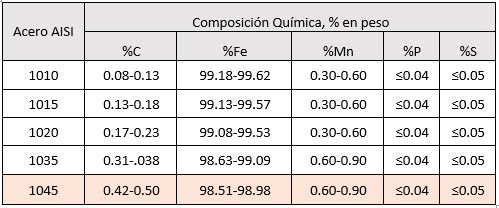
\includegraphics[scale=0.5]{tablaacero.jpg}
  \caption{Clasificaci\'on de aceros de acuerdo a la norma AISI \cite{ref1}.}
  \label{tab}
\end{figure}

\section{Antecedentes}

Las metalograf\'ias son im\'agenes tomadas de la superficie de una muestra que son visibles mediante un microscopio, estas im\'agenes han sido ampliamente utilizadas para conocer la microestructura con mayor detalle. La microestructura puede presentar diversas fases que han sido reconocidas a trav\'es de los diagramas de fase, en los que se representan las temperaturas y los porcentajes en composici\'on en los que se logran formar dichas fases (figura 2). Cada fase tiene una concentraci\'on distinta de las dem\'as por lo que tambi\'en sus propiedades son diferentes y con ello las posibles aplicaciones del material\cite{ref5}. 

\begin{figure}[H]
  \centering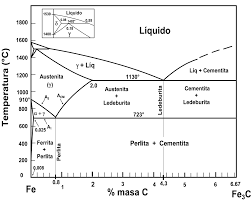
\includegraphics[scale=0.6]{diagramaFeC.png}
  \caption{Diagrama de fases de Hierro-Carbono \cite{ref8}.}
  \label{fig}
\end{figure}

Cada microestructura presenta una forma granular, debido a que todos los metales solidos son cristalinos por su naturaleza, procedente de la formaci\'on de peque\~n os cristales en el metal fundido durante el proceso de solidificaci\'on \cite{ref1}.
Las simulaciones computacionales han sido utilizadas en el procesamiento de im\'agenes digitales para lograr una adecuada apreciaci\'on y correcta interpretaci\'on de estas, en el caso de los aceros se han logrado analizar fases como la ferrita, martensita, perlita, etc. Diversos lenguajes de programaci\'on han sido utilizados con este prop\'osito, as\'i como para el estudio de otros materiales, siendo los mas atractivos los softwares libres de c\'odigo abierto\cite{ref3} \cite{ref4}.


\section{Trabajos Relacionados}
Diversos autores han utilizado el procesamiento de im\'agenes mediante alg\'un software con el prop\'osito de usarlo para micrograf\'ias. A continuaci\'on, se muestra el cuadro 1  en el que se mencionan las caracter\'isticas principales de sus trabajos.

\begin{table}[H]
\centering
\caption{Comparaci\'on de trabajos relacionados}
\begin{tabular}{rrr}

\hline
Autor&Aportac\'ion\\
\hline
\textit{Castro M.}\cite{ref6}&Paquetes ITK y VTK\\
\textit{Silva A.}\cite{ref3}& Fundiciones nodulares\\
\textit{Llulluna F.}\cite{ref2}&Uso de multilenguaje\\
\textit{Chiriboga C.}\cite{ref4}&Gr\'aficas Ashby\\

\hline
\end{tabular}
\label{t1}
\end{table}


\section{Soluci\'on propuesta}

Mediante el uso de una micrograf\'ia previamente realizada en una muestra de acero se intenta determinar cu\'ales son las fases presentes, esto se puede lograr mediante un c\'odigo que al seleccionar una imagen pueda detectar los pixeles dentro de ella y generar un histograma que brinde la informaci\'on mencionada. Posteriormente se compara los resultados con los datos encontrados en la literatura y as\'i evaluar la similitud del experimento.

\subsection{Metodolog\'ia}

Para el desarrollo del an\'alisis metalogr\'afico se requiri\'o del programa Python 3 con el cual, a trav\'es del uso de la librer\'ia OpenCv fue posible analizar la imagen seccion\'andola a partir de los pixeles de la imagen utilizada, este tipo de im\'agenes normalmente son presentadas en escala de grises, esto con el objetivo de generar un mayor contraste y una mejor visualizaci\'on de la microestructura. Para determinar la cantidad de pixeles que es encontraban en la escala de grises fue necesario usar la descripci\'on RGB (del ingl\'es Red ``Rojo'', Green  ``Verde'' y Blue  ``Azul'') que hace referencia a la composici\'on del color en t\'erminos de la intensidad de los colores primarios con que se forma: el rojo, el verde y el azul. Es un modelo de color basado en la s\'intesis aditiva, con el que es posible representar un color mediante la mezcla por adici\'on de los tres colores primarios.
El modelo RGB indica la proporci\'on en que se mezclan cada uno de los tres colores, se asigna un valor para cada uno, de modo que el valor 0 indica que el color no intervino en la mezcla, y el valor 255 indica que es la m\'axima intensidad del color proporcionado, de manera mas explicita se muestra la figura 3, donde se marca el color negro como la ausencia de los tres componentes (0, 0, 0) y el color blanco como el m\'aximo nivel (255, 255, 255) \cite{ref7}.

\begin{figure}[H]
  \centering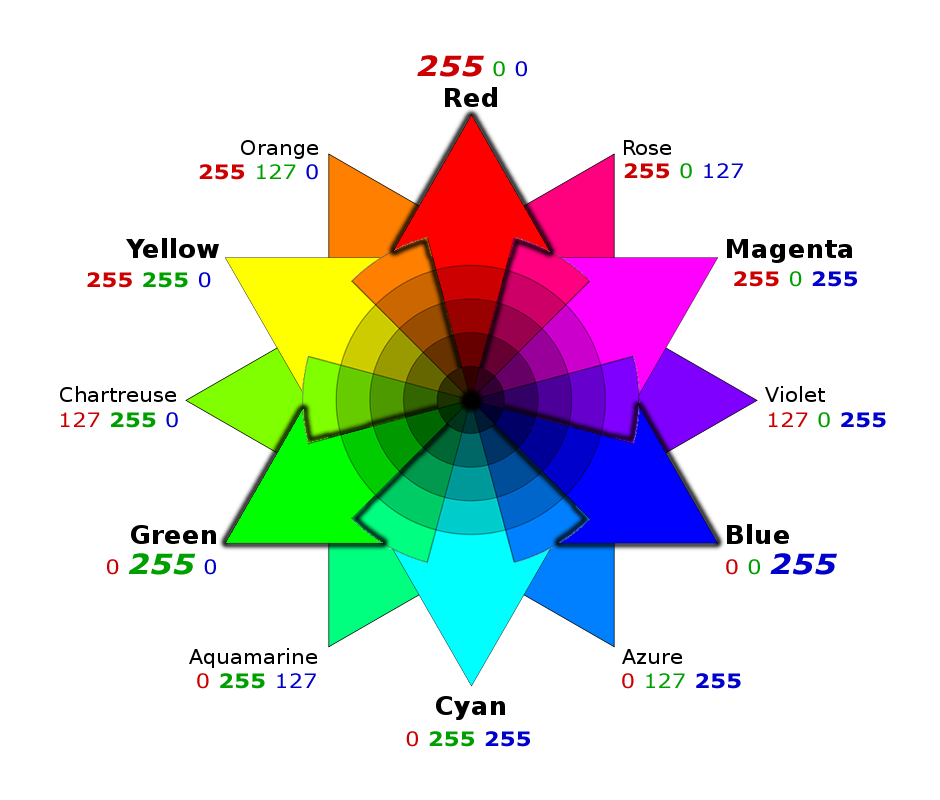
\includegraphics[scale=0.15]{coloresrgb.png}
  \caption{Valores de los colores formados en la escala RGB \cite{ref7}.}
  \label{fig}
\end{figure}

Con base en la imagen \cite{metal2}en escala de grises de un acero 1045 \cite{ref1} se obtuvo un histograma en la que se encuentra graficada la intensidad con respecto a la cantidad de pixeles que se encuentran en la imagen y a partir de la cual se busc\'o determinar la cantidad en la que se presentaban las fases. V\'ease figura 4.

\begin{figure}[H]
       \centering
       \begin{subfigure}[b]{0.4\linewidth}
           \includegraphics[width=\linewidth]{metal2.jpg}
           \label{fig:westminster_lateral}
        \end{subfigure}

        \begin{subfigure}[b]{0.6\linewidth}
            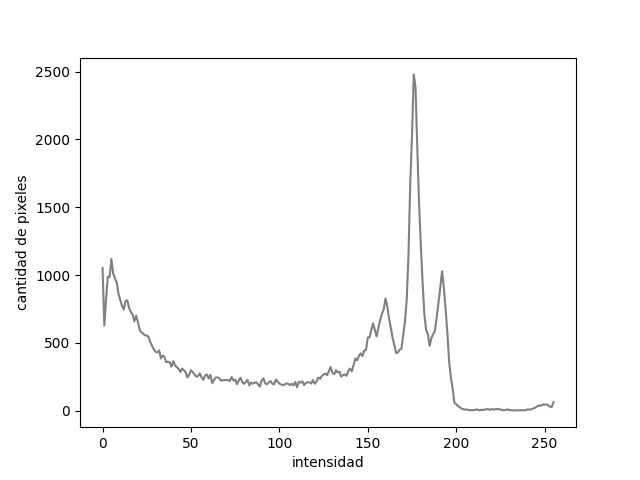
\includegraphics[width=\linewidth]{histograma2.png}
            \label{fig:westminster_lateral}
         \end{subfigure}
         \caption{Im\'agen de la microestructura y su correspondiente histograma \cite{metal}.}
\end{figure}

El mismo procedimiento fue realizado en otras dos im\'agenes a manera de comprobaci\'on. V\'eanse figuras 5 y 6.

\begin{figure}[H]
       \centering
       \begin{subfigure}[b]{0.4\linewidth}
           \includegraphics[width=\linewidth]{metal1.jpg}
           \label{fig:westminster_lateral}
        \end{subfigure}

        \begin{subfigure}[b]{0.6\linewidth}
            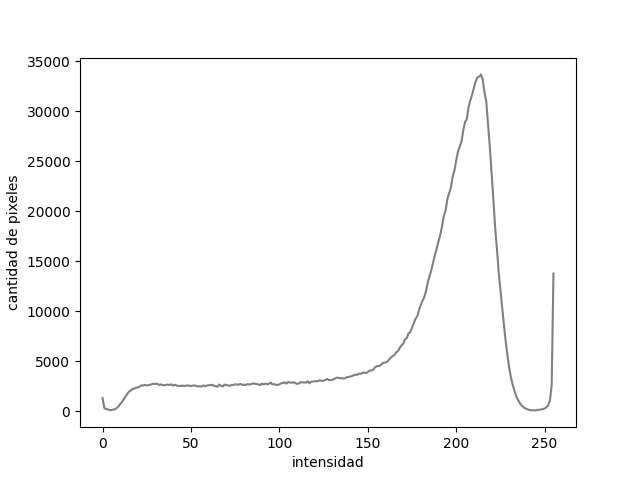
\includegraphics[width=\linewidth]{histograma1.png}
            \label{fig:westminster_lateral}
         \end{subfigure}
         \caption{Im\'agen de la microestructura y su correspondiente histograma\cite{metal2}.}
\end{figure}

\begin{figure}[H]
       \centering
       \begin{subfigure}[b]{0.4\linewidth}
           \includegraphics[width=\linewidth]{metal3.jpg}
           \label{fig:westminster_lateral}
        \end{subfigure}

        \begin{subfigure}[b]{0.6\linewidth}
            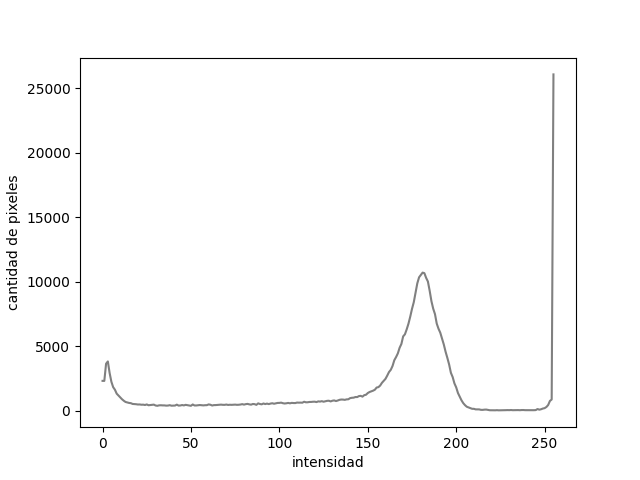
\includegraphics[width=\linewidth]{histograma3.png}
            \label{fig:westminster_lateral}
         \end{subfigure}
         \caption{Im\'agen de la microestructura y su correspondiente histograma \cite{metal}.}
\end{figure}

\section{Evaluaci\'on}

Como se mencion\'o anteriormente, fue necesario comparar los resultados y la manera m\'as pr\'actica fue mediante un an\'alisis ANOVA. A continuaci\'on, se muestran los resultados obtenidos (figuras 7 y 8).
\begin{figure}[H]
  \centering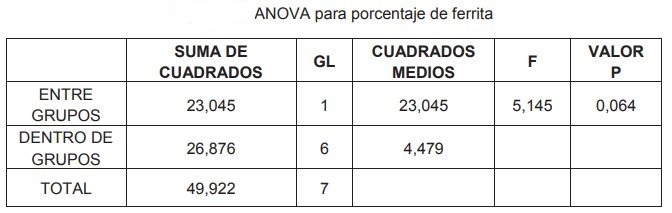
\includegraphics[scale=0.4]{anova1.jpg}
  \caption{An\'alisis anteriormente reportado \cite{ref2}.}
  \label{fig}
\end{figure}

\begin{figure}[H]
  \centering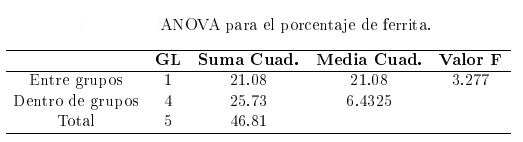
\includegraphics[scale=0.6]{anova2.jpg}
  \caption{An\'alisis obtenido.}
  \label{fig}
\end{figure}
\subsection{Dise\~no experimental}
La simulaci\'on fue llevada a cabo en Python Shell en la que se mostraba el histograma de la imagen analizada, posteriormente el histograma fue usado como referencia para la integraci\'on del \'area generada y se procedi\'o al an\'alisis de los datos para su comparaci\'on. Esta simulaci\'on fue aplicada en un procesador \textcopyright{Intel Celeron} N2840 con el uso de 4GB de memoria RAM por lo que es recomendable tomar en cuenta las condiciones de uso para una mejor eficiencia.
La escala RGB fue ajustada de manera que detectara los tonos de gris presentes en la imagen y as\'i generar el histograma para posteriormente proceder a ser comparadas con los datos existentes.

\section{Conclusiones}

En el an\'alisis metalogr\'afico de una pieza de acero fue necesario para conocer su microestructura y saber as\'i que propiedades podr\'ia presentar, para dicho an\'alisis se requiri\'o del software libre Python con el que se buscaba identificar la(s) fase(s) presentes y as\'i auxiliarnos de un m\'etodo simple y capaz de reproducirse en diferentes muestras.

Los datos obtenidos durante el experimento se\~nalan que se obtuvo una aproximaci\'on adecuada a la reportada por la literatura, lo que permite su implementaci\'on como herramienta auxiliar en el campo de la metalurgia tradicional, sabiendo que el posible resultado es aproximado al de los determinados con softwares especializados.

La fase ferrita fue identificada en la imagen reportada por \cite{metal} y comparada con la reportada por \cite{ref2} lo que siguiere un adecuada experimentaci\'on.

\section{Trabajos Futuros}

El campo de la metalurgia es muy amplio y requiere de muchos procesos en los que se realizan an\'alisis de datos obtenidos a partir de im\'agenes, como en el caso de las micrograf\'ias en superaleaciones y de aleaciones no ferrosas en la que se busca determinar tanto composici\'on como posibles defectos e inclusiones en la muestra adem\'as de extenderse a campos como la cer\'amica en la que se requiere conocer porcentajes de porosidad, la implementaci\'on de un software libre ayuda al desarrollo de m\'etodos m\'as sencillos que permitan, entre otras cosas, facilitar la caracterizaci\'on de este tipo de materiales.

\section{Agradecimientos}

Agradezco a la Dra. Elisa Schaeffer por su ayuda durante la realizaci\'on de este trabajo y el material de apoyo\cite{satuelisa}\cite{doctora}, as\'i como sus ense\~nanzas durante el curso de simulaci\'on computacional de nanomateriales en el semestre agosto 2020 -- enero 2021.

\bibliography{proyecto}
\bibliographystyle{unsrtnat}


\end{document}